\chapter{Probability}
This course will use probability theory quite a lot, but we will often use
a fairly informal notation. Bayesian
statistics is really just probability theory used for a particular purpose --
to describe uncertainty. The two most important rules of probability are given below.

\section{The Product Rule}
The first important rule of probability is the
product rule. This tells us how to calculate the probability that any two
propositions or hypotheses $A$ and $B$ are {\bf both} true.
The probability of $P$ {\bf and}
$B$ will be denoted $P(A, B)$. This can be calculated by first finding the
probability that $A$ is true, and then multiplying by the probability that $B$
is true {\it given} that $A$ is true.
\begin{eqnarray}
P(A, B) &=& P(A)P(B|A)\label{product1}
\end{eqnarray}
We could also have done this the other way around: first finding the
probability that $B$ is true and then the probability that $A$ is true given
that $B$ is true:
\begin{eqnarray}
P(A, B) &=& P(B)P(A|B).\label{product2}
\end{eqnarray}
You may be familiar with the idea of a {\it tree diagram} from earlier
statistics courses or maybe even high school. A tree diagram is a helpful way
to work with the product rule. If you find tree diagrams helpful, feel free to
use them, although tree diagrams themselves will not be examinable.

\begin{figure}[ht!]
\begin{center}
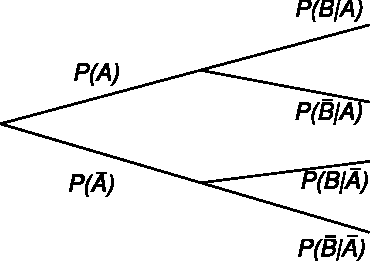
\includegraphics[scale=0.9]{Figures/tree_diagram.pdf}
\caption{\it A tree diagram.}
\end{center}
\end{figure}

\subsection{Bayes' Rule}
Looking at Equations~\ref{product1} and~\ref{product2}, they are both equations
for the same
thing, $P(A,B)$. Therefore we can equate the right hand sides. Doing this gives
a result known as Bayes' rule:
\begin{eqnarray}
P(A|B) &=& \frac{P(A)P(B|A)}{P(B)}. \label{bayes}
\end{eqnarray}
Bayes' rule will be used extensively throughout this course. You will need to
know it and know how to use it!

\section{The Sum Rule}
The sum rule is the second important rule of probability. It is used to obtain
the probability that some proposition $A$ is true from some other
probabilities. Say we want the probability of $A$ but to do that, we would need
to know the status (truth or falsehood) of some other statement $B$. Then we
can use the sum rule:
\begin{eqnarray}
P(A) &=& P(A, B) + P(A, \bar{B})\\
&=& P(B)P(A|B) + P(\bar{B})P(A|\bar{B}).
\end{eqnarray}
where the over-bar means ``not'', i.e. $\bar{B}$ means $B$ is false. To understand
this formula, imagine we want to know the probability of $A$. Well there are
two mutually exclusive ways that could happen: via $B$ being true, or via $B$
being false. The first way has probability $P(B)P(A|B)$, and the second way
has probability $P(\bar{B})P(A|\bar{B})$.

In Bayesian statistics the sum rule is most often used to calculate the
normalising constant $P(D)$, and it is also used to marginalise out ``nuisance
parameters'', although in STATS 331 we will mostly use MCMC to do the latter.

\section{Random Variables}
Throughout this course I will use the term ``probability distribution'' to
refer to both the probability mass function for a discrete random variable, and
the probability density function for a continuous random variable. I will also
use a common shorthand notation.

\subsection{Discrete Random Variables}
We will also see quite a lot of random variables in this course (although
without using that terminology very much as I consider the word ``random'' to be
worse than useless). A discrete
random variable is just a quantity $X$ that has a countable number of possible
values. A discrete random variable has a {\it probability mass function}
that tells you, as a function of the {\it possible} values $x$.
For example, the equation for the Poisson distribution (a useful discrete
distribution) is:
\begin{eqnarray}
P(X=x) &=& \frac{\lambda^x e^{-\lambda}}{x!}\label{eq:poisson}
\end{eqnarray}
for $x \in \{0, 1, 2, 3, ...\}$. The actual random variable is named $X$, and
$x$ is just used so we can write the probabilities ($P(X=0), P(X=1), ...)$ as
a formula.

\subsection{Continuous Random Variables}
Continuous random variables are those where the set of possibilities is
continuous. For example, with a normal distribution, technically any real value
is possible. Therefore it doesn't make sense to ask, for example, the probability
that $X=1.32$: the answer is zero because the total probability of 1 has to be
spread among an infinite number of possibilities. Instead we can ask the probability
that $X$ is in some region that has a nonzero size. In general, if $X$ has a
probability density function $f(x)$, then the probability that $X \in [a, b]$ is:
\begin{eqnarray}
P(a \leq X \leq b) &=& \int_a^b f(x) \, dx.
\end{eqnarray}
Note the lower case $x$ in the probability density function: this is analogous
to the lower case $x$ in the probability mass function of a discrete random
variable. Note that I won't often get you to do an integral analytically. One
of the major reasons why MCMC is so awesome is that you can get away without
having to do hard integrals!

\subsection{Shorthand Notation}
The notation of random variables can be cumbersome. For example, consider
inferring a (discrete) parameter $Y$ from (discrete) data $X$. Bayes' rule gives us:
\begin{eqnarray}
P(Y=y | X=x) &=& \frac{P(Y=y)P(X=x|Y=y)}{P(Y=y)}.
\end{eqnarray}
That's very verbose, so instead we use the shorthand:
\begin{eqnarray}
p(y | x) &=& \frac{p(y)p(x|y)}{p(y)}.
\end{eqnarray}
In this notation we don't distinguish between the symbol for the random variable
and the dummy variables that allow us to write the probability distribution as
a formula, we just use the lower case for everything. Despite this simplification,
everything still works. Just read
$p(y|x)$ as ``the probability distribution for $y$ given $x$'' and everything
will be fine. Astute readers may have noticed that when I gave the Poisson formula
(Equation~\ref{eq:poisson}), ``given $\lambda$'' was implicit throughout.

To be clear when we are talking about a simple probability and when we are
talking about the probability distribution for a variable, I will use upper case
$P$ for the former and lower-case $p$ for the latter.

\section{Useful Probability Distributions}
In the course we will study Bayesian models which involve the following
discrete probability distributions: general (all probabilities given explicitly,
such as in a Bayes' Box), binomial, Poisson, discrete uniform,
negative binomial, multinomial.
We may also use the following continuous distributions: uniform, normal,
Cauchy, student-$t$, beta, log-uniform, exponential, gamma, Dirichlet.

Wikipedia is an excellent resource for looking up all the properties of these
distributions, but I will also give various properties (e.g. the mean of a beta
distribution) and describe the distributions when we need them.

